\part{Разработка програмного обеспечения}

Как правило систематическое занесение доходов и расходов в таблицу, а
также подсчет итогового баланса может оказаться весьма непростым занятием, но и использование электронных таблиц и специализированных программ
тоже не тривиальная задача, поскольку такие методы разрабатываются с учетом максимально широких возможностей использования, от самых простых
табличных расчетов и до учета дивидендов от приобретенных акций, что не
очень хорошо ложится на базовый семейный бюджет.

\section{Разработка базовой концепции приложения}
В качестве базовой концепции приложения был выбран вариант модифицированных электронных таблиц. Самым простым вариантом была следующая структура
\begin{enumerate}
	\item Размер операции
	\item "Сторона"операции (приход/расход)
	\item Коментарий к операции
	\item Дата и время операции
\end{enumerate}

Остаток вычислялся путем последовательного суммирования (с модификатором "стороны") размеров операции отсортированных по датам и времени
операции

\subsection{Начало разработки}
Первоначальная версия сущестовала в консольном виде без взаимодействия с курсором мыши. Данные хранились в текстовом виде, что позволяло
легко модифицировать записанные данные. Позже были добавлены категории записей, которые позволили однозначно делать подсчет расходов по категориям расходов.

\section{Разработка графической версии}
Немного позже был разработан первоначальный вариант графической версии приложения, он по прежнему записывал данные в файл и при этом работал достаточно неэффективно.

\begin{figure}[H]
	\centering
	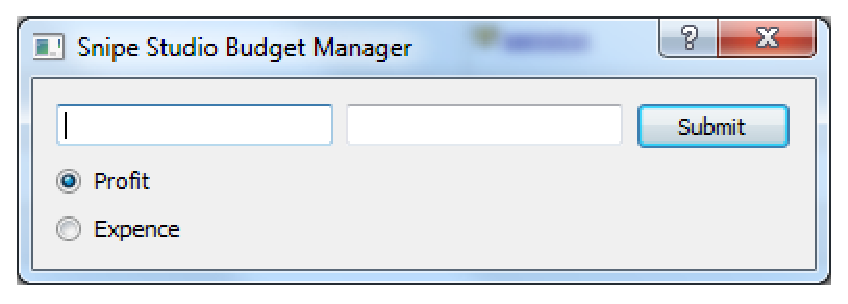
\includegraphics[width=0.7\linewidth]{pics/firstVersion.eps}
	\caption{Первоначальный вариант графического приложения Budget Manager}
	\label{fig:firstVersion}
\end{figure}

Немного позднее было добавлено поле отображающее список операций

\begin{figure}[H]
	\centering
	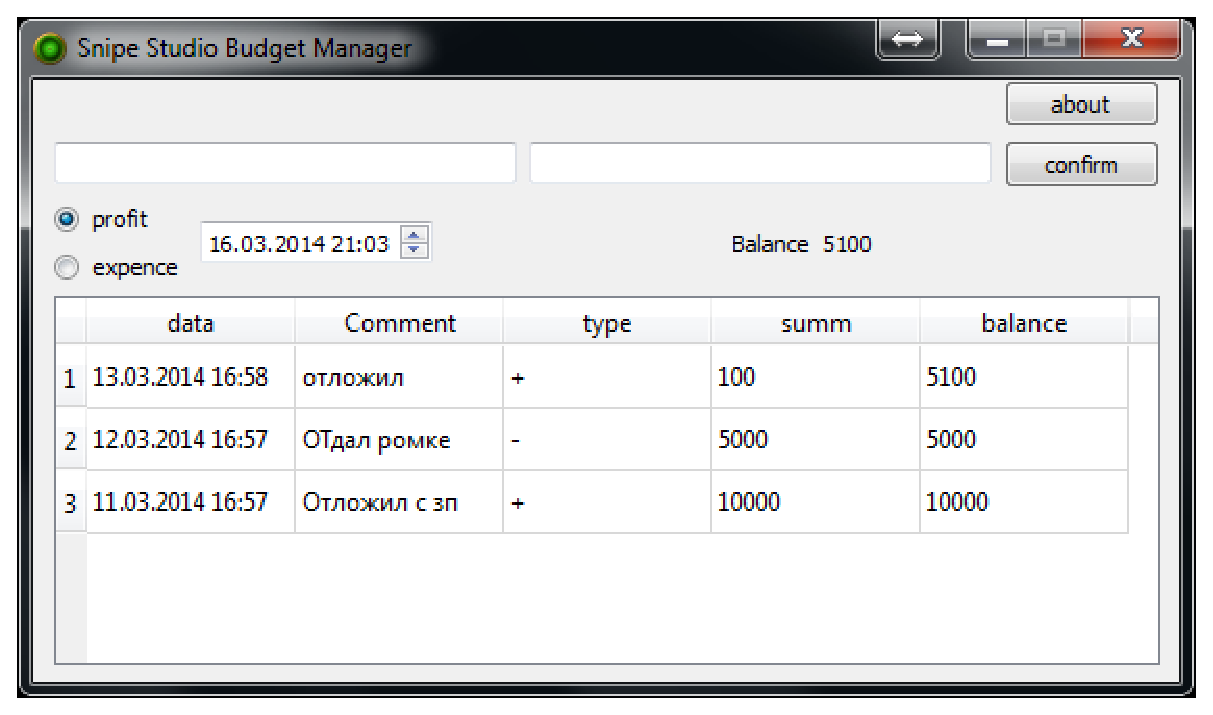
\includegraphics[width=0.7\linewidth]{pics/secondVersion.eps}
	\caption{Вариант графического приложения Budget Manager с таблицей со списком
		операции}
	\label{fig:secondVersion}
\end{figure}

Дальше был изменен метод хранения и изменения уже существующих записей, добавлено полноценное меню настроек, строки таблицы теперь окрашиваются в зависимости от выбраной "стороны"(приход/расход) для операции

\begin{figure}[H]
	\centering
	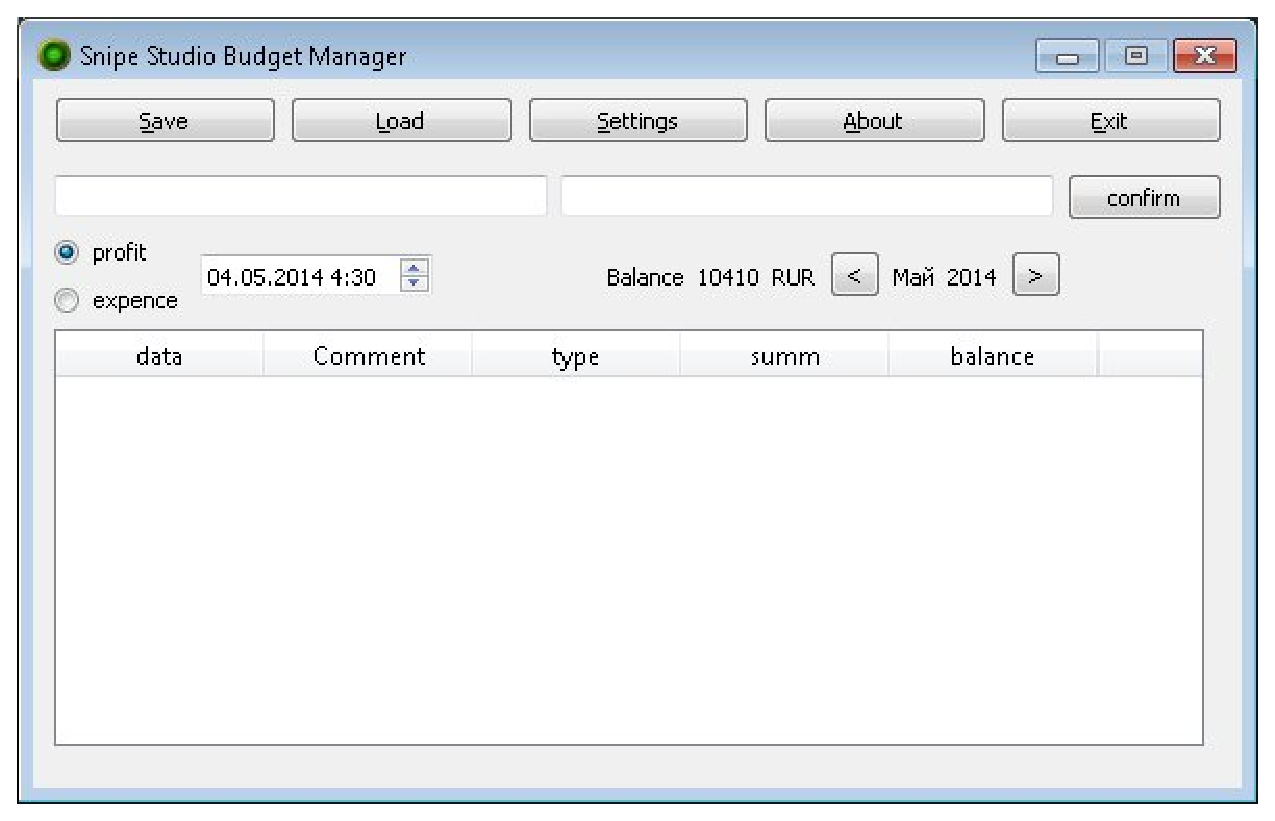
\includegraphics[width=0.7\linewidth]{pics/view1.eps}
	\caption{Окончательный вариант графического приложения Budget Manager}
	\label{fig:view1}
\end{figure}

Позже был изменен общий графический дизайн приложения 	и стал следующим:

\begin{figure}[H]
	\centering
	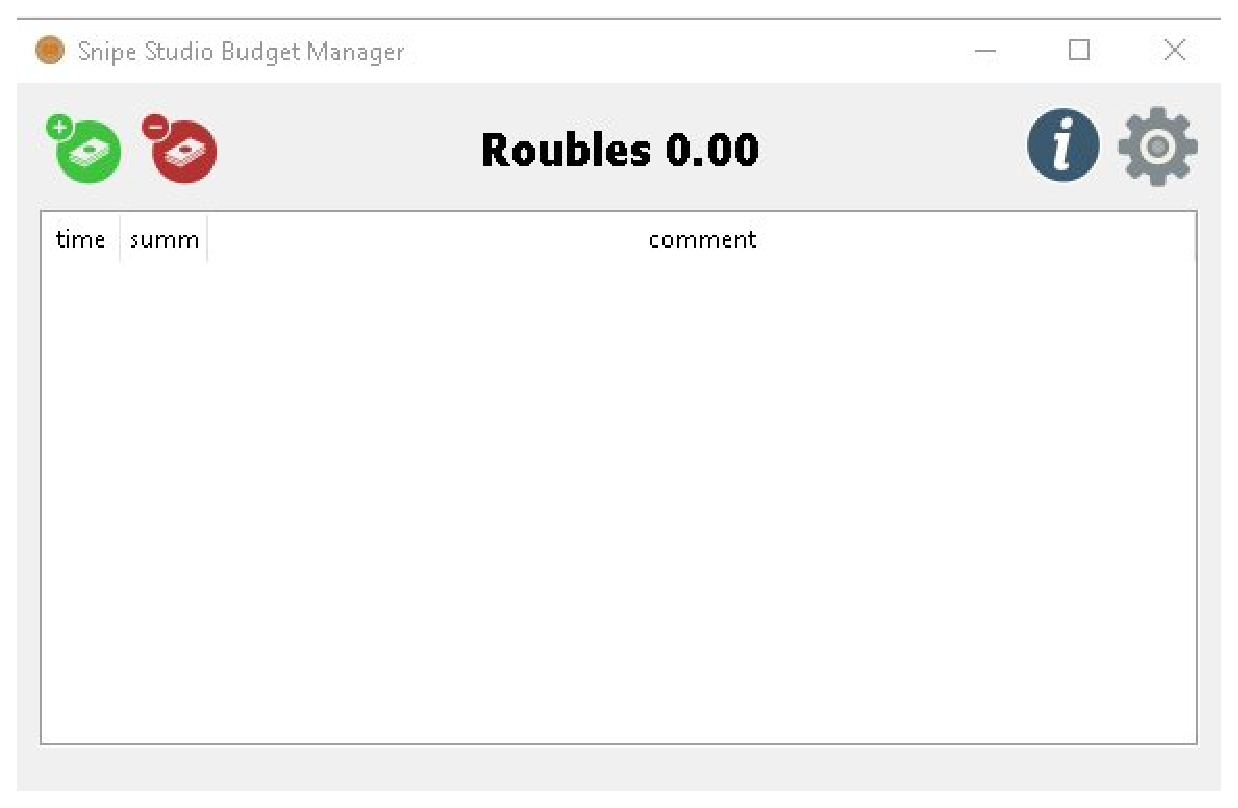
\includegraphics[width=0.7\linewidth]{pics/view2.eps}
	\caption{Второй вариант графического приложения Budget Manager}
	\label{fig:view2}
\end{figure}

Так же была собрана версия для Android

\begin{figure}[H]
	\centering
	
	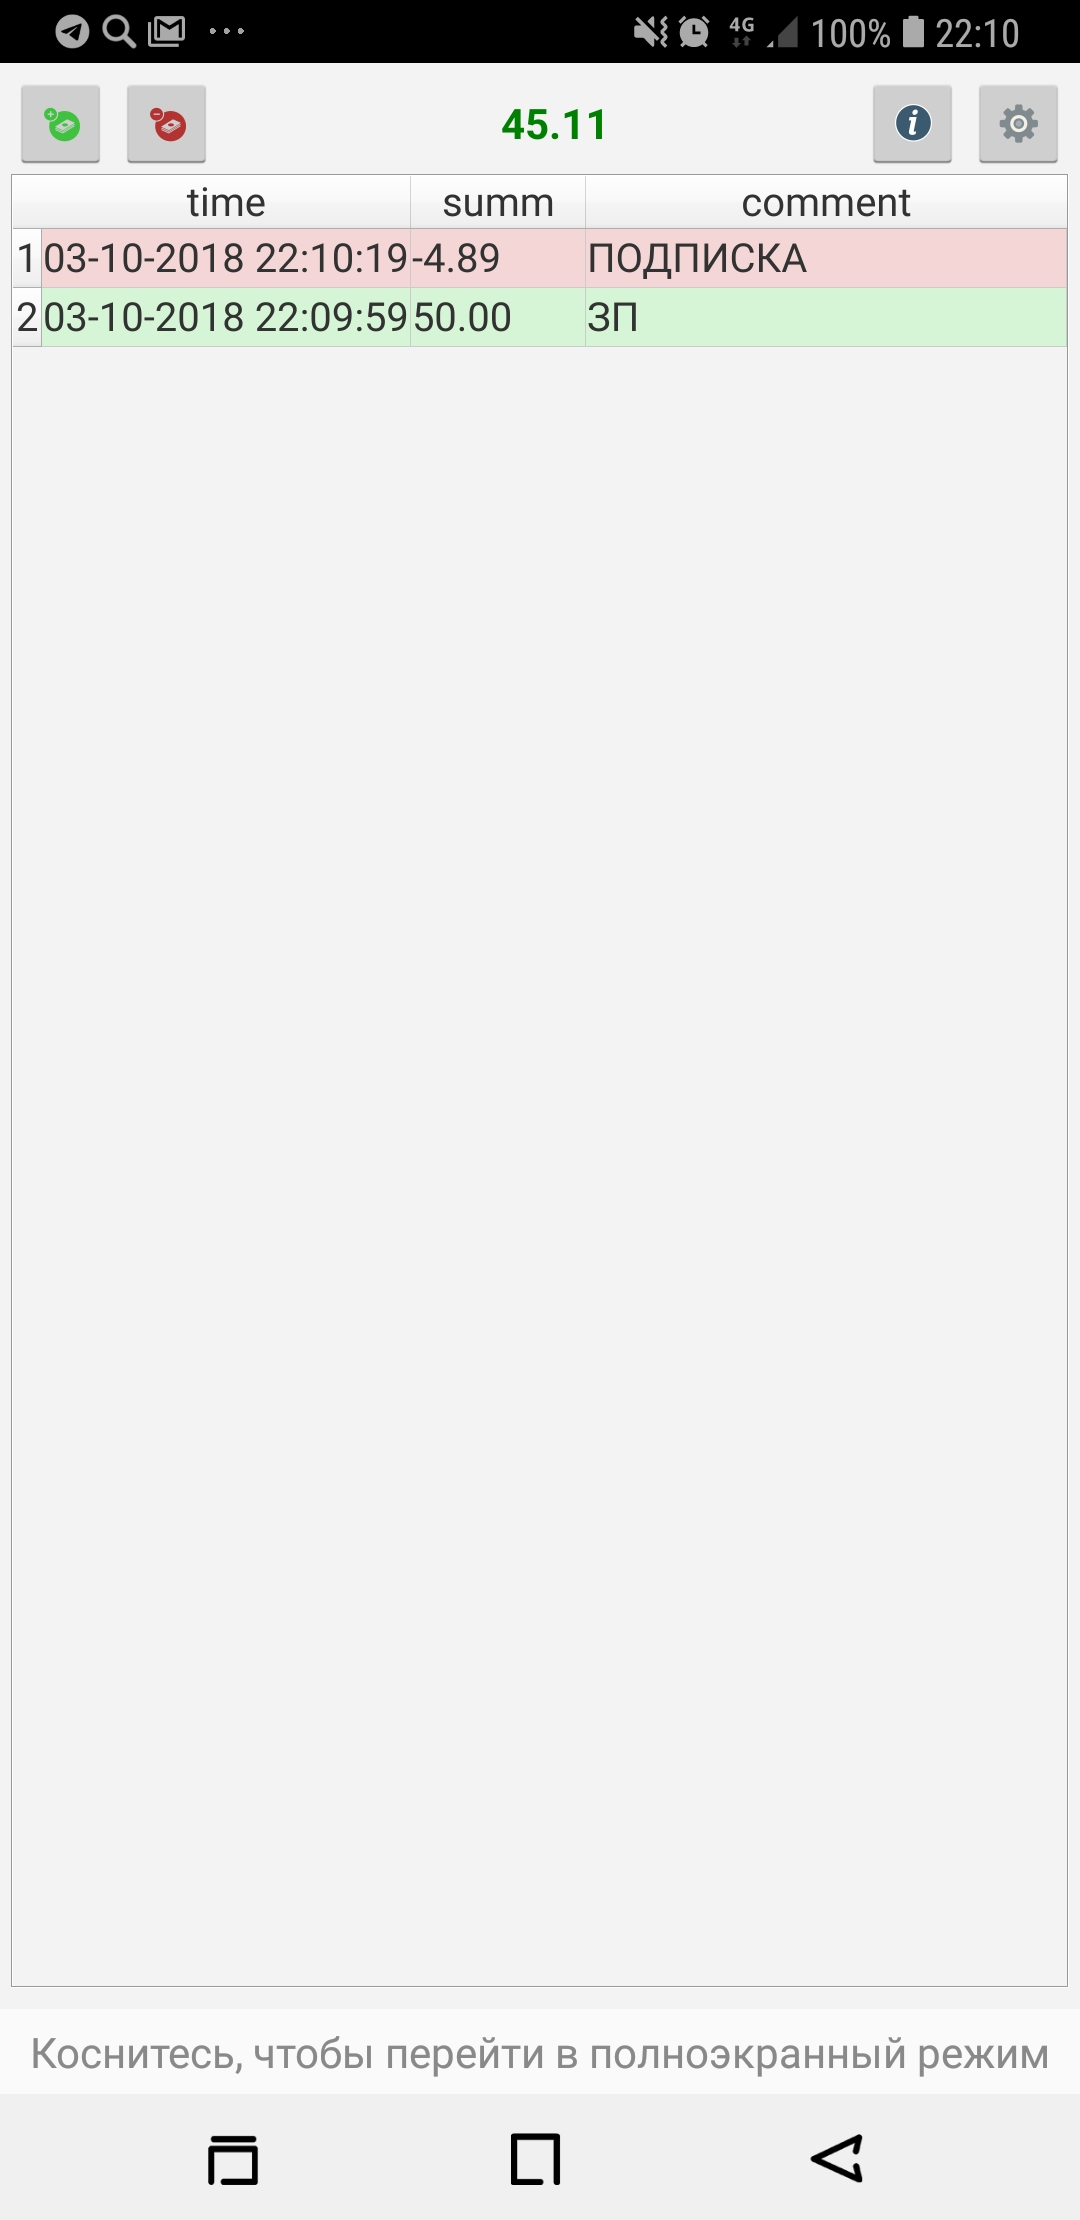
\includegraphics[height=0.7\linewidth]{pics/viewAndroid.eps}
	\caption{Версия для Android}
	\label{fig:viewAndroid}
\end{figure}

\section{Автоматизированная сборка и тестирование}
Спустя некоторое время мне понадобилось автоматически собирать инсталляторы для каждого коммита, чтобы не тратить каждый раз время на полноценную сборку инсталлятора и deb-пакета для приложения. Для этих целей я выбрал Azure DevOps, который предоставлял бесплатные сборочные машины и целую готовую инфраструктуру для автоматизированной сборки и тестирования.\\
Для целей автоматизированного тестирования был создан интерфейс командной строки, который позволяет использовать все возможности приложения без необходимости запускать графический интерфейс пользователя, что позволило тестировать приложения в операционных системах без графической среды пользователя.\\
\subsection{Автоматическая сборка}
Сборочная цепочка для AzureDevops под операционную систему Linux на базе Ubuntu 16.04 имеет следующий вид:
\begin{figure}[H]
	\centering
	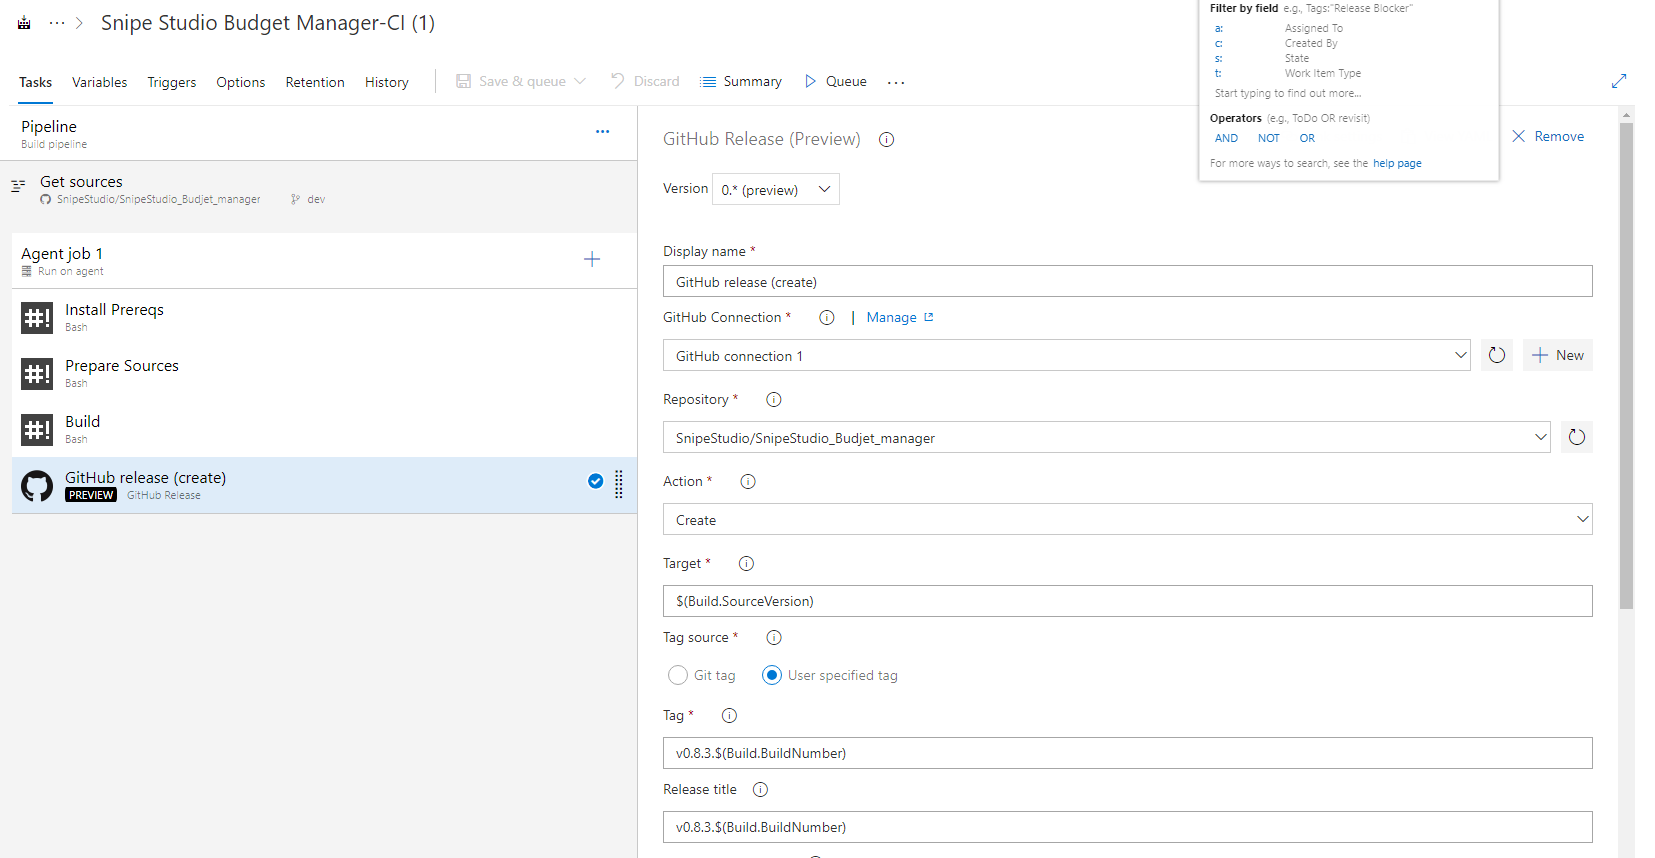
\includegraphics[width=1\linewidth]{pics/AzurePipeline.eps}
	\caption{Azure Pipeline}
	\label{fig:AzurePipeline}
\end{figure}

В шаге Install Prereqs происходит установка QT для возможности сборки приложения.\\
Prepare Sources заменяет версию в Файле appinfo.h на текущую версию приложения, т.е. имеет вид 0.8.3.(buildNumber)\\
Шаг Build осуществляет сборку бинарного файла приложения\\
Шаг GitHub Release публикует PreRelease версию на GitHub с указанием тага текущей сборки\\
\begin{figure}[H]
	\centering
	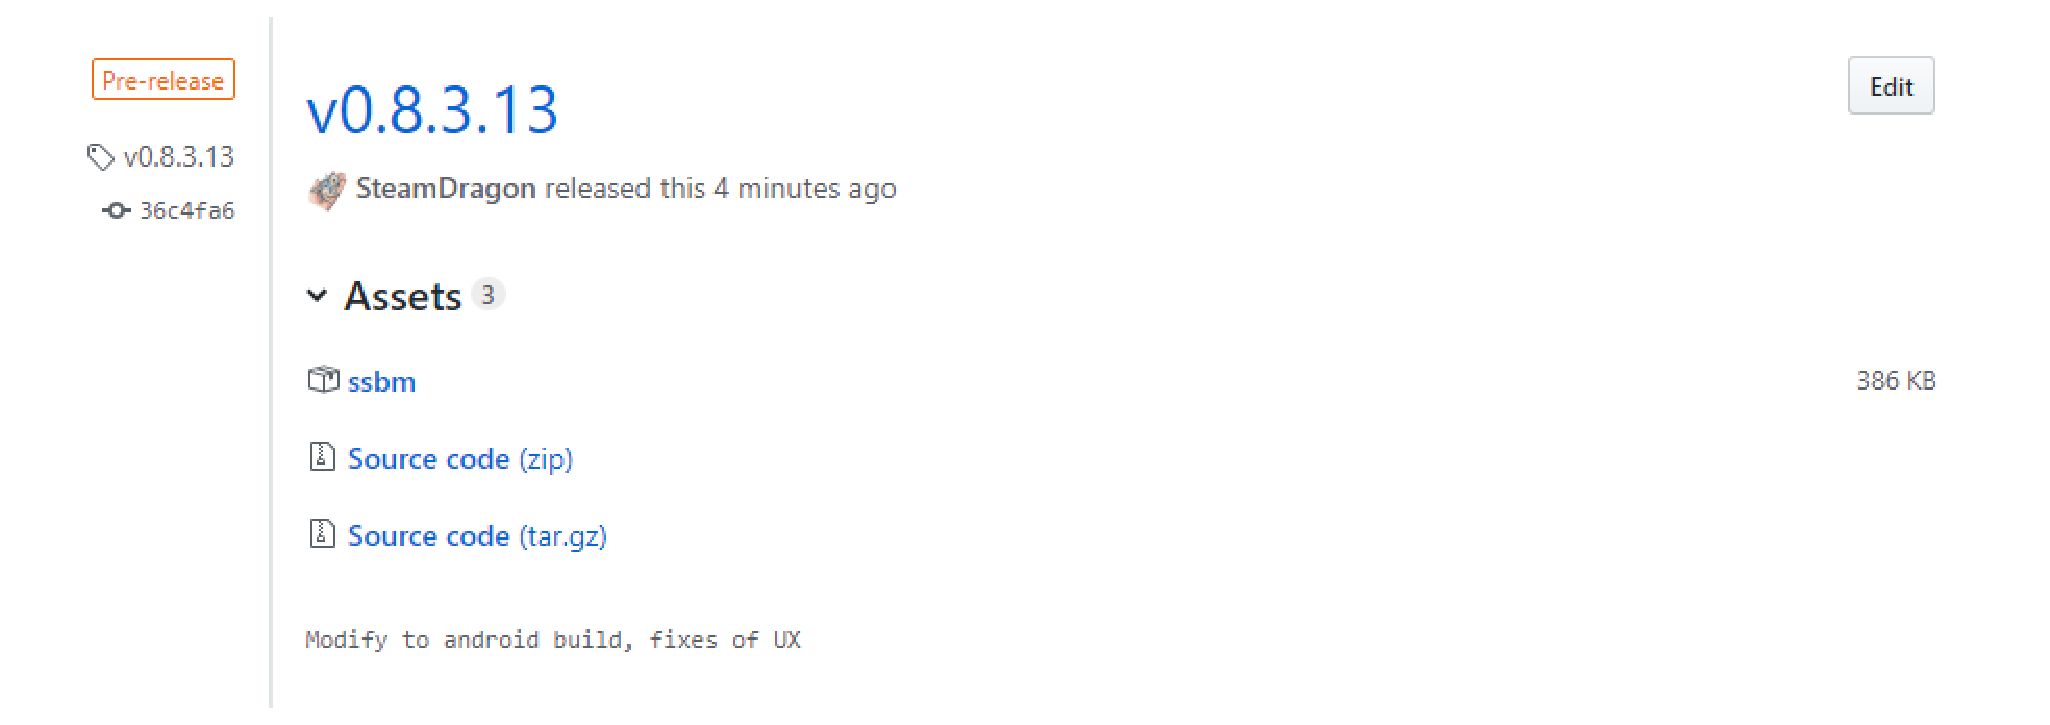
\includegraphics[width=1\linewidth]{pics/GHRelease.eps}
	\caption{Github Release}
	\label{fig:GHRelease}
\end{figure}
Сборка под операционную систему Windows имеет ту же структуру, что и сборка под Ubuntu, за одним исключением, версия сборки берется из сборки для Ubuntu.
\subsection{Автоматизированное Тестирование}
Автоматизированное тестирование программного обеспечения — часть процесса тестирования на этапе контроля качества в процессе разработки программного обеспечения. Оно использует программные средства для выполнения тестов и проверки результатов выполнения, что помогает сократить время тестирования и упростить его процесс. \cite{AutoTest}

Для обеспечения корректной и стабильной работы были разработаны автоматизированные тесты на основе Google Test Framework (Google C++ Testing Framework (Google Test) — библиотека для модульного тестирования (англ. unit testing) на языке С++. Исходные тексты открыты с середины 2008 года под лицензией BSD. Документация частично переведена на русский язык.

Google Test построена на методологии тестирования xUnit, то есть когда отдельные части программы (классы, функции, модули) проверяются отдельно друг от друга, в изоляции. Библиотека сама по себе разработана с активным применением тестирования, когда при добавлении каких-либо частей в официальную версию, кроме кода самих изменений необходимо написать набор тестов, подтверждающих их корректность.)\cite{GTest} Был подготовлен ряд автоматизированных xUnit-тестов для каждого функционального элемента программы, для целей полноценного функционирования автотестов, а так же возможности использования приложения в окружениях без возможности использования GUI был подготовлен интерфейс взаимодействия командной строки. Работа с командной строкой осуществлялась с помощью класса commandLine и библиотеки QComandLineParser входящую в пакет поставки QT начиная с версии 5.8.0\\

Каждая возможная опция представляется в следующем виде
\begin{MyCode}
	QCommandLineOption* exportOption = new QCommandLineOption(
	QStringList() << "e"  
	<< "export",          
	QCoreApplication::translate("main", 
	"Exporting database to <file>."), 
	QCoreApplication::translate("main", "file"));
\end{MyCode}

QCoreApplication::translate позволяет использовать текст, указанный в его параметрах в качестве источника материала для локализации приложения. \\
В параметры QCommandLineOption  передается список строк со следующей структурой: "Краткая команда", "Полная Команда", "Описание команды, которое будет высвечено при запросе справки приложения в командной строке", "параметр, который будет учтен в данной команде"\\
